% https://tex.stackexchange.com/q/759062/322482
\documentclass[tikz,border=5pt]{standalone}
\usepackage{fourier}
\begin{document}

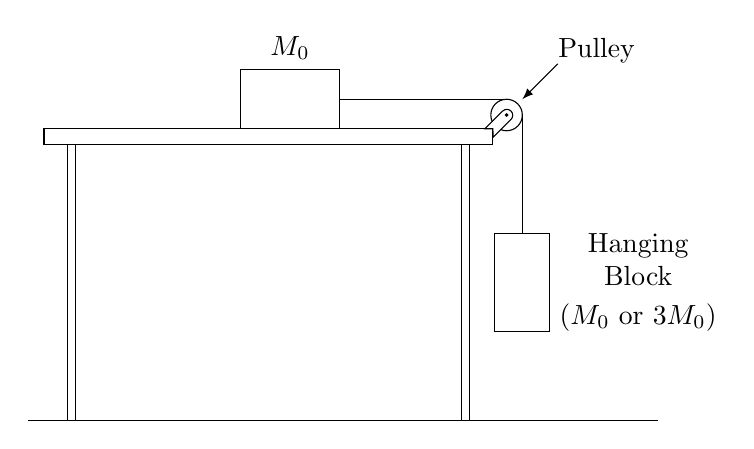
\begin{tikzpicture}
    \coordinate (L) at (.5,0);
    \coordinate (R) at (5.5,0);
    \draw (0,0) -- ++(8,0);
    \draw (L) rectangle ++(.1,3.5)
          (R) rectangle ++(.1,3.5) % desk legs
          ++(.3,.2) coordinate (corner)
          rectangle ++(-5.7,-.2) % desktop
          ++(2.5,.2) rectangle ++(1.25,.75) 
          node[midway,above=.375cm] {$M_0$} % box on the desktop
          ++(0,-.375) coordinate (line)
          ;
    \path (corner) 
        ++(.375,.375) coordinate (pulley) % 
        ++(-.2,-.2) coordinate (center) % pulley radius=.2
        ;
    \draw (center) circle[radius=.2]; % pulley drawing
    \fill[white,draw=black] (corner) ++(-.1,0) -- ++(.225,.225) arc[start angle=135,delta angle=-180,radius=.075] -- ++(-.225,-.225) -- (corner) --cycle;
    \fill (center) circle[radius=.025]; % pulley center drawing
    \path[draw] 
        (line) -- (center|-line) 
        (pulley|-center) -- ++(0,-1.5) 
        ++(-.35,0) rectangle ++(.7,-1.25) 
        node[pos=.5,right=.35cm,align=center] {Hanging\\Block\\[2pt]($M_0$ or $3M_0$)}
        ;
    \draw[-latex] (pulley) ++ (.45,.45) node[inner sep=0pt,anchor=south west] {Pulley} -- (pulley) ;
\end{tikzpicture}

\end{document}